%%%%%%%%%%%%%%%%%%%%%%%%%%%%%%%%%%%%
% Slide options
%%%%%%%%%%%%%%%%%%%%%%%%%%%%%%%%%%%%

% Option 1: Slides with solutions

\documentclass[slidestop,compress,mathserif]{beamer}
\newcommand{\soln}[1]{\textit{#1}}
\newcommand{\solnGr}[1]{#1}
\usepackage{booktabs}

% Option 2: Handouts without solutions

%\documentclass[11pt,containsverbatim,handout]{beamer}
%\usepackage{pgfpages}
%\pgfpagesuselayout{4 on 1}[letterpaper,landscape,border shrink=5mm]
%\newcommand{\soln}[1]{ }
%\newcommand{\solnGr}{ }

\def\argmax{\operatornamewithlimits{arg\,max}}
\def\argmin{\operatornamewithlimits{arg\,min}}

%%%%%%%%%%%%%%%%%%%%%%%%%%%%%%%%%%%%
% Style
%%%%%%%%%%%%%%%%%%%%%%%%%%%%%%%%%%%%
%%%%%%%%%%%%%%%%%%%%%%%%%%%%%%%%%%%%%%%%%%%%%%%%%%%%%%%%%%%%%%%%%%%%%%%%
% MA213/214 shared slide style
%
% "Calm & Cool" palette + content-type callout boxes.
% Overhauled (2026) from the original OpenIntro/metropolis style:
%   - all OpenIntro visual branding removed (logo, grid, colors)
%   - a low-key cool palette (see colors below)
%   - tcolorbox callout boxes so students recognize content types
% See common/README.md for the command cheat-sheet.
%%%%%%%%%%%%%%%%%%%%%%%%%%%%%%%%%%%%%%%%%%%%%%%%%%%%%%%%%%%%%%%%%%%%%%%%

\usetheme{metropolis}

%%%%%%%%%%%%%%%%
% Packages
%%%%%%%%%%%%%%%%

\usepackage{geometry}
\usepackage{graphicx}
\usepackage{amssymb}
\usepackage{epstopdf}
\usepackage{amsmath}  	% this permits text in eqnarray among other benefits
\usepackage{url}		% produces hyperlinks
\usepackage{hyperref}	% allows for color usage in tables
\usepackage[english]{babel}
\usepackage[latin1]{inputenc}
\usepackage{colortbl}	% allows for color usage in tables
\usepackage{multirow}	% allows for rows that span multiple rows in tables
\usepackage{color}		% this package has a variety of color options
\usepackage{pgf}
\usepackage{calc}
\usepackage{ulem}
\usepackage{multicol}
\usepackage{textcomp}
\usepackage{txfonts}
\usepackage{listings}
\usepackage{tikz}
\usepackage{array}
\usepackage{wasysym}
\usepackage{fancyvrb}
\usepackage{etoolbox}             % \ifstrempty for optional box subtitles
\usepackage[most]{tcolorbox}      % content-type callout boxes
\tcbuselibrary{listings}          % R-code block (\begin{rblock})
\usepackage{fontawesome5}         % box icons

%%%%%%%%%%%%%%%%
% Remove navigation symbols
%%%%%%%%%%%%%%%%

\setbeamertemplate{navigation symbols}{}

%%%%%%%%%%%%%%%%
% "Calm & Cool" palette
%%%%%%%%%%%%%%%%

% chrome / structure / body
\definecolor{ccSlate}{HTML}{2E3742}   % frametitle bar, structure, section pages (deep neutral slate)
\definecolor{ccInk}{HTML}{2B2B2B}     % body text
\definecolor{ccWash}{HTML}{FCF8F1}    % gentle warm title-slide background wash (complements the cool blues)

% example (blue)
\definecolor{ccBlue}{HTML}{2F6690}
\definecolor{ccBlueBg}{HTML}{EAF1F7}
% interactive activity / discussion (green)
\definecolor{ccGreen}{HTML}{4E8A6B}
\definecolor{ccGreenBg}{HTML}{E9F3EC}
% solution (purple)
\definecolor{ccPurple}{HTML}{6F5499}
\definecolor{ccPurpleBg}{HTML}{EFEAF6}
% worksheet / focused work (terracotta)
\definecolor{ccTerra}{HTML}{C2693E}
\definecolor{ccTerraBg}{HTML}{FAEDE4}
% formula / definition (neutral slate)
\definecolor{ccGray}{HTML}{5C6B7A}
\definecolor{ccGrayBg}{HTML}{EEF1F4}
% caution / common pitfall (brick red)
\definecolor{ccRed}{HTML}{B23A48}
\definecolor{ccRedBg}{HTML}{FAEAEC}
% key idea / takeaway (muted gold)
\definecolor{ccGold}{HTML}{9C7A28}
\definecolor{ccGoldBg}{HTML}{F7F1DF}
% learning goals / lesson outcomes (teal)
\definecolor{ccTeal}{HTML}{2C6E6B}
\definecolor{ccTealBg}{HTML}{E6F0EF}
% learning objectives (indigo)
\definecolor{ccIndigo}{HTML}{45507A}
\definecolor{ccIndigoBg}{HTML}{ECEEF4}
% R code / output (gray)
\definecolor{ccCode}{HTML}{5F5E5A}
\definecolor{ccCodeBg}{HTML}{F4F5F6}

% neutral grays kept from the original style
\definecolor{gray}{rgb}{0.5, 0.5, 0.5}
\definecolor{darkGray}{rgb}{0.3, 0.3, 0.3}
\definecolor{darkerGray}{rgb}{0.2, 0.2, 0.2}

% Backwards-compatible aliases: old OpenIntro color names now point at the
% new palette, so existing \textcolor{oiB}{...}, \hl{...}, etc. keep working.
\colorlet{oiB}{ccBlue}
\colorlet{oiG}{ccGreen}
\colorlet{hlblue}{ccBlue}
\colorlet{rubineRed}{ccRed}
\colorlet{irishGreen}{ccGreen}
\colorlet{lightGreen}{ccGreen}

%%%%%%%%%%%%%%%%
% Restyle metropolis with the Calm & Cool chrome
%%%%%%%%%%%%%%%%

\metroset{block=fill}

\setbeamercolor{normal text}{fg=ccInk, bg=white}
\setbeamercolor{structure}{fg=ccSlate}
\setbeamercolor{alerted text}{fg=ccBlue}
\setbeamercolor{example text}{fg=ccGreen}
\setbeamercolor{frametitle}{bg=ccSlate, fg=white}
\setbeamercolor{progress bar}{fg=ccBlue}
\setbeamercolor{title separator}{fg=ccBlue}
\setbeamercolor{title}{fg=ccSlate}
\setbeamercolor{subtitle}{fg=ccBlue}
\setbeamercolor{author}{fg=ccInk}
\setbeamercolor{institute}{fg=ccGray}
\setbeamercolor{date}{fg=ccGray}
\setbeamercolor{section title}{fg=ccSlate}
\setbeamercolor{standout}{fg=white, bg=ccSlate}

% Section pages sit on the same warm wash as the title slide. We keep
% metropolis's section-title styling and just paint a full-page ccWash
% background behind it (needs >=2 pdflatex passes for the current-page node).
\setbeamertemplate{section page}{%
  \begin{tikzpicture}[remember picture, overlay]
    \fill[ccWash] (current page.south west) rectangle (current page.north east);
  \end{tikzpicture}%
  \centering
  \begin{minipage}{22em}
    \raggedright
    \usebeamercolor[fg]{section title}%
    \usebeamerfont{section title}%
    \insertsectionhead\\[-1ex]
    \usebeamertemplate*{progress bar in section page}%
    \par
  \end{minipage}\par
  \vspace{\baselineskip}
}

%%%%%%%%%%%%%%%%
% Custom inline text commands (recolored to the palette)
%%%%%%%%%%%%%%%%

% degree
\newcommand{\degree}{\ensuremath{^\circ}}

% cite
\newcommand{\ct}[1]{
\vfill
{\tiny #1}}

\newcommand{\NamedNote}[2]{
\rule{2.5cm}{0.25pt} \\ \textit{\footnotesize{\textcolor{rubineRed}{#1:} \textcolor{darkerGray}{#2}}}}

% Note
\newcommand{\Note}[1]{
\rule{2.5cm}{0.25pt} \\ \textit{\footnotesize{\textcolor{rubineRed}{Note:} \textcolor{darkerGray}{#1}}}}

% Remember
\newcommand{\Remember}[1]{\textit{\scriptsize{\textcolor{ccTerra}{Remember:} #1}}}

% expected counts
\newcommand{\ex}[1]{\textit{\textcolor{ccBlue}{#1}}}

% red
\newcommand{\red}[1]{\textit{\textcolor{rubineRed}{#1}}}

% pink
\newcommand{\pink}[1]{\textit{\textcolor{rubineRed!90!white!50}{#1}}}

% green
\newcommand{\green}[1]{\textit{\textcolor{irishGreen}{#1}}}

% orange
\newcommand{\orange}[1]{\textit{\textcolor{ccTerra}{#1}}}

% links: webURL, webLink, appLink
\newcommand{\webURL}[1]{\urlstyle{same}{ \textit{\textcolor{darkGray}{\url{#1}}}}}
\newcommand{\webLink}[2]{\href{#1}{\textcolor{darkGray}{{#2}}}}
\newcommand{\appLink}[2]{\href{#1}{\textcolor{white}{{#2}}}}

% mail
\newcommand{\mail}[1]{\href{mailto:#1}{\textit{\textcolor{darkGray}{#1}}}}

% highlighting: hl, hlGr, mathhl
\newcommand{\hl}[1]{\textit{\textcolor{hlblue}{#1}}}
\newcommand{\hlGr}[1]{\textit{\textcolor{lightGreen}{#1}}}
\newcommand{\mathhl}[1]{\textcolor{hlblue}{\ensuremath{#1}}}

%%%%%%%%%%%%%%%%
% Structural helpers (unchanged from the original)
%%%%%%%%%%%%%%%%

% two col: two columns
\newenvironment{twocol}[4]{
\begin{columns}[c]
\column{#1\textwidth}
#3
\column{#2\textwidth}
#4
\end{columns}
}

% slot (for probability calculations)
\newenvironment{slot}[2]{
\begin{array}{c}
\underline{#1} \\
#2
\end{array}
}

% pr: left and right parentheses
\newcommand{\pr}[1]{
\left( #1 \right)
}

% cancel
\newcommand{\cancel}[1]{%
    \tikz[baseline=(tocancel.base)]{
        \node[inner sep=0pt,outer sep=0pt] (tocancel) {#1};
        \draw[red, line width=0.5mm] (tocancel.south west) -- (tocancel.north east);
    }%
}

% removepagenumbers
\newcommand{\removepagenumbers}{%
  \setbeamertemplate{footline}{}
}

% change margin
\newenvironment{changemargin}[2]{%
\begin{list}{}{%
\setlength{\topsep}{0pt}%
\setlength{\leftmargin}{#1}%
\setlength{\rightmargin}{#2}%
\setlength{\listparindent}{\parindent}%
\setlength{\itemindent}{\parindent}%
\setlength{\parsep}{\parskip}%
}%
\item}{\end{list}}

% footnote
\long\def\symbolfootnote[#1]#2{\begingroup%
\def\thefootnote{\fnsymbol{footnote}}\footnote[#1]{#2}\endgroup}

% commands from the book
\newenvironment{data}[1]{\texttt{#1}}{}
\newenvironment{var}[1]{\texttt{#1}}{}
\newenvironment{resp}[1]{\texttt{#1}}{}

%%%%%%%%%%%%%%%%
% Content-type callout boxes (tcolorbox)
%
% Each type has a colored title strip (icon + label) over a light fill.
% Color = content type; the label + icon reinforce it (so the cue does
% not rely on color alone).
%%%%%%%%%%%%%%%%

\tcbset{
  cccallout/.style 2 args={
    enhanced, breakable=false,
    colback=#2, colframe=#1, colbacktitle=#1, coltitle=white,
    fonttitle=\bfseries\footnotesize,
    boxrule=0.6pt, arc=2.5pt, outer arc=2.5pt,
    left=5pt, right=5pt, top=3pt, bottom=3pt, boxsep=2pt,
    toptitle=2pt, bottomtitle=2pt, lefttitle=5pt,
    before skip=5pt, after skip=5pt,
  },
}

% One-off / collection of examples (blue): \workedexample[subtitle]{body}.
% (Named \workedexample, not \example, because beamer defines \example.)
\newtcolorbox{examplebox}[1][]{cccallout={ccBlue}{ccBlueBg},
  title={\faIcon{lightbulb}~~Example\ifstrempty{#1}{}{ \textmd{---}\ #1}}}
\newcommand{\workedexample}[2][]{\begin{examplebox}[#1]#2\end{examplebox}}

% Running-example header (blue): \examplehead{name} at the top of each frame of a
% multi-slide running example. A one-off or a collection of examples uses the
% \workedexample box above instead.
\newcommand{\examplehead}[1]{%
  \vspace{-0.4em}\par\noindent\tcbox[on line, colback=ccBlue, colframe=ccBlue, coltext=white,
    boxrule=0pt, arc=2pt, left=5pt, right=5pt, top=1pt, bottom=1pt,
    box align=base, nobeforeafter]{\footnotesize\bfseries\faIcon{lightbulb}\,Running example}%
  \ifstrempty{#1}{}{\enspace{\footnotesize\bfseries\textcolor{ccBlue}{#1}}}%
  \par\nobreak\vspace{-0.6em}{\color{ccBlue}\rule{\linewidth}{0.7pt}}\par\nobreak\vspace{-0.8em}}

% Interactive activity (green): \activity[subtitle]{body}
\newtcolorbox{activitybox}[1][]{cccallout={ccGreen}{ccGreenBg},
  title={\faIcon{users}~~Activity\ifstrempty{#1}{}{ #1}}}
\newcommand{\activity}[2][]{\begin{activitybox}[#1]#2\end{activitybox}}

% Discussion question (green): \dq{body}
\newtcolorbox{dqbox}{cccallout={ccGreen}{ccGreenBg}, title={\faIcon{comments}~~Discussion}}
\newcommand{\dq}[1]{\begin{dqbox}#1\end{dqbox}}

% Solution (purple): \solnbox{body}. Gated by the per-deck \soln toggle, so it
% shows in the instructor build and vanishes from the student handout build.
% (Named \solnbox, not \solution, because beamer already defines \solution.)
\newtcolorbox{solutionbox}{cccallout={ccPurple}{ccPurpleBg}, title={\faIcon{key}~~Solution}}
\newcommand{\solnbox}[1]{\soln{\begin{solutionbox}#1\end{solutionbox}}}

% Worksheet / focused work (terracotta): \worksheet[subtitle]{body}
\newtcolorbox{worksheetbox}[1][]{cccallout={ccTerra}{ccTerraBg},
  title={\faIcon{pencil-alt}~~Worksheet\ifstrempty{#1}{}{ #1}}}
\newcommand{\worksheet}[2][]{\begin{worksheetbox}[#1]#2\end{worksheetbox}}

% Formula / definition (neutral slate). Supports both real usages found in the
% decks: \formula{title}{body} and the bare \formula{body} (title defaults to
% "Formula"). The second group is an optional brace argument.
\newtcolorbox{formulabox}[1][Formula]{cccallout={ccGray}{ccGrayBg},
  title={\faIcon{square-root-alt}~~#1}}
\NewDocumentCommand{\formula}{m g}{%
  \IfNoValueTF{#2}%
    {\begin{formulabox}#1\end{formulabox}}%
    {\begin{formulabox}[#1]#2\end{formulabox}}}

% Common pitfall / caution (brick red): \caution[subtitle]{body}
\newtcolorbox{cautionbox}[1][]{cccallout={ccRed}{ccRedBg},
  title={\faIcon{exclamation-triangle}~~Caution\ifstrempty{#1}{}{ #1}}}
\newcommand{\caution}[2][]{\begin{cautionbox}[#1]#2\end{cautionbox}}

% Key idea / takeaway (muted gold): \keyidea[subtitle]{body}
\newtcolorbox{keyideabox}[1][]{cccallout={ccGold}{ccGoldBg},
  title={\faIcon{star}~~Key idea\ifstrempty{#1}{}{ #1}}}
\newcommand{\keyidea}[2][]{\begin{keyideabox}[#1]#2\end{keyideabox}}

% Learning goals / lesson outcomes (teal): \goals{body}. Sits under the short
% LO headings on the objectives slide; body is the "you should be able to" list.
\newtcolorbox{goalsbox}{cccallout={ccTeal}{ccTealBg}, fontupper=\footnotesize,
  top=1pt, bottom=2pt, boxsep=1pt, before skip=3pt,
  title={\faIcon{bullseye}~~By the end of today, you should be able to\ldots}}
\newcommand{\goals}[1]{\begin{goalsbox}#1\end{goalsbox}}

% Learning objectives (indigo): \objectives{body} -- the formal LO headings,
% shown alongside \goals on the objectives slide.
\newtcolorbox{objectivesbox}{cccallout={ccIndigo}{ccIndigoBg}, fontupper=\small,
  top=1pt, bottom=2pt, boxsep=1pt, before skip=3pt,
  title={\faIcon{clipboard-list}~~Learning objectives}}
\newcommand{\objectives}[1]{\begin{objectivesbox}#1\end{objectivesbox}}

% Defaults for a bare \begin{lstlisting}. Without these it inherits the listings
% package defaults: 11pt type, fixed-width columns (which spaces code out as
% "a g e _ f i t"), and no line breaking, so a long line silently runs off the
% right edge of the slide. A deck that passes its own basicstyle still wins.
% Layout only -- syntax coloring is left to the \begin{rblock} environment.
\lstset{
  basicstyle=\ttfamily\footnotesize, columns=fullflexible,
  breaklines=true, breakindent=1.5em, showstringspaces=false,
  numbers=none, frame=none}

% R code / output (gray): \begin{rblock}[subtitle] ... \end{rblock}
% NOTE: a frame containing an rblock must be declared \begin{frame}[fragile].
\lstdefinestyle{ccR}{
  language=R, basicstyle=\ttfamily\footnotesize, columns=fullflexible,
  breaklines=true, showstringspaces=false, numbers=none, frame=none,
  keywordstyle=\color{ccBlue}, commentstyle=\color{ccGreen!75!black},
  stringstyle=\color{ccTerra}}
\newtcblisting{rblock}[1][]{cccallout={ccCode}{ccCodeBg},
  title={\faIcon{terminal}~~R\ifstrempty{#1}{}{ #1}},
  listing only, listing style=ccR}

% --- Legacy boxes (kept so existing decks compile) ---

% app: application exercise -> alias of activity
\newcommand{\app}[1]{\activity{#1}}

% pq: practice question (green, interactive family)
\newtcolorbox{pqbox}{cccallout={ccGreen}{ccGreenBg}, title={\faIcon{list-ol}~~Practice}}
\newcommand{\pq}[1]{\begin{pqbox}#1\end{pqbox}}

% solnMult: solutions for multiple-choice practice questions (uses \soln toggle)
\newcommand{\solnMult}[1]{
\item[] \vspace{-0.59cm}
\only<1>{\item #1}
\soln{\only<2->{\item \orange{#1}}}
}

%%%%%%%%%%%%%%%%
% De-branded title frame + attribution
%%%%%%%%%%%%%%%%

% Eyebrow line on the title slide; a deck may \renewcommand this.
\newcommand{\coursetag}{MA214: Applied Statistics}

% Attribution: all slides released under CC BY-SA, crediting both the
% instructor (later material) and OpenIntro (basis of the earlier material).
\newcommand{\courseattribution}{%
  Slides by Jonathan H.~Huggins, building on materials from OpenIntro's
  \emph{Introduction to Modern Statistics} (Mine \c{C}etinkaya-Rundel et al.).
  Released under the
  \webLink{http://creativecommons.org/licenses/by-sa/3.0/us/}{CC BY-SA license}.
  Some images included under fair use (educational purposes).}

% \maketitleframe: de-branded title slide (no logo, no grid). Uses the deck's
% \title, \subtitle, and \coursetag.
\newcommand{\maketitleframe}{%
  \addtocounter{framenumber}{-1}%
  {\removepagenumbers
  \setbeamercolor{background canvas}{bg=ccWash}%
  \begin{frame}[plain]
    \vspace*{2.6em}
    {\color{ccSlate}\rule{\textwidth}{2.5pt}}\par\vspace{1.5em}
    {\usebeamerfont{date}\scshape\color{ccGray}\coursetag}\par\vspace{0.55em}
    {\usebeamerfont{title}\color{ccSlate}\inserttitle\par}
    \vspace{0.45em}{\color{ccBlue}\rule{3em}{2.5pt}}\par\vspace{0.7em}
    {\usebeamerfont{subtitle}\color{ccBlue}\insertsubtitle\par}
    \vfill
    {\color{ccGray!55}\rule{\textwidth}{0.4pt}}\par\vspace{0.45em}
    {\tiny\color{ccGray}\courseattribution\par}
    \vspace*{0.4em}
  \end{frame}}}

%%%%%%%%%%%%%%%%
% Graphics
%%%%%%%%%%%%%%%%

\DeclareGraphicsRule{.tif}{png}{.png}{`convert #1 `dirname #1`/`basename #1 .tif`.png}

\graphicspath{ {../../common/} }


%%%%%%%%%%%%%%%%%%%%%%%%%%%%%%%%%%%%
% Preamble
%%%%%%%%%%%%%%%%%%%%%%%%%%%%%%%%%%%%

\title[Lecture 8]{Lecture 8: Hypothesis testing with randomization}
\subtitle{Module 2: Statistical Inference}
\author{Introduction to Modern Statistics, 2nd Edition}
\institute{$\:$ \\ {\footnotesize Based on slides developed by Mine \c{C}etinkaya-Rundel of OpenIntro.  \\
The slides may be copied, edited, and/or shared via the \webLink{http://creativecommons.org/licenses/by-sa/3.0/us/}{CC BY-SA license.} \\
Some images may be included under fair use guidelines (educational purposes).}}
\date{}

%%%%%%%%%%%%%%%%%%%%%%%%%%%%%%%%%%%%
% Begin document
%%%%%%%%%%%%%%%%%%%%%%%%%%%%%%%%%%%%

\begin{document}


%%%%%%%%%%%%%%%%%%%%%%%%%%%%%%%%%%%%
% Title page
%%%%%%%%%%%%%%%%%%%%%%%%%%%%%%%%%%%%

\maketitleframe

% !TEX root =  Lecture8.tex


%%%%%%%%%%%%%%%%%%%%%%%%%%%%%%%%%%%%
% Recap/Agenda
%%%%%%%%%%%%%%%%%%%%%%%%%%%%%%%%%%%%
\begin{frame}
\frametitle{Module 2: Statistical Inference}
    \begin{itemize}
    \item \hl{Previously:} Module 1 --- building, interpreting, and choosing regression models.
    \item \hl{This time:} \emph{how sure are we?} Testing with randomization.
      \begin{itemize}
      \item statistics, sampling distributions, and the null distribution
      \item hypothesis testing review, p-values, and decision errors
      \item building the null distribution by \hl{randomization}
      \end{itemize}
    \item \hl{Reading:} IMS Chapters 11 and 14.
    \item \hl{Homework for today:}
    \item \hl{Homework for next class:}
    \end{itemize}
\end{frame}


%%%%%%%%%%%%%%%%%%%%%%%%%%%%%%%%%%%%
% Learning objectives:
%%%%%%%%%%%%%%%%%%%%%%%%%%%%%%%%%%%%
\begin{frame}
    \frametitle{Lecture Objectives}
    \goals{%
    \begin{itemize}
    \item explain what a sampling distribution is, and what makes the \emph{null} distribution the one we can build;
    \item state hypotheses, choose a test statistic, and interpret a p-value correctly;
    \item distinguish Type I from Type II errors and say which one matters in context;
    \item given a null hypothesis, determine \emph{what to randomize} --- and carry out the test.
    \end{itemize}}
    \objectives{%
    \begin{itemize}
    \item \textbf{(M2, LO1)} Approaches to Inference
    \item \textbf{(M2, LO2)} Simulation-based Inference
    \end{itemize}}
\end{frame}


%%%%%%%%%%%%%%%%%%%%%%%%%%%%%%%%%%%%%%%%%%%%%%%%%%%%%%%%%%%%%%%%%%%%%%%%
\section{From estimates to uncertainty}
%%%%%%%%%%%%%%%%%%%%%%%%%%%%%%%%%%%%%%%%%%%%%%%%%%%%%%%%%%%%%%%%%%%%%%%%
\begin{frame}
\frametitle{Module 1 gave us numbers. How sure are we?}

Over seven lectures we produced a lot of numbers:
\[
\widehat\beta_1 = -0.62,
\qquad
e^{\hat\beta} = 4.94,
\qquad
R^2_{adj} = 0.26,
\qquad
\text{AIC} = 57.3 .
\]
Every one of them is a \hl{point estimate} computed from \emph{one} sample.

\pause
\begin{itemize}
\item Draw a different sample (other states, other people) and every one of those numbers changes.
\item So which differences are \emph{real}, and which are just the luck of the sample?
\end{itemize}

\pause
\vspace{-0.3em}
\keyidea[-- Module 2]{Inference turns a number computed from one sample into a statement about the population, \emph{with its uncertainty attached}.}

\end{frame}
%%%%%%%%%%%%%%%%%%%%%%%%%%%%%%%%%%%%%%%%%%%%%%%%%%%%%%%%%%%%%%%%%%%%%%%%
\begin{frame}
\frametitle{The big picture: closing the loop}

\begin{center}
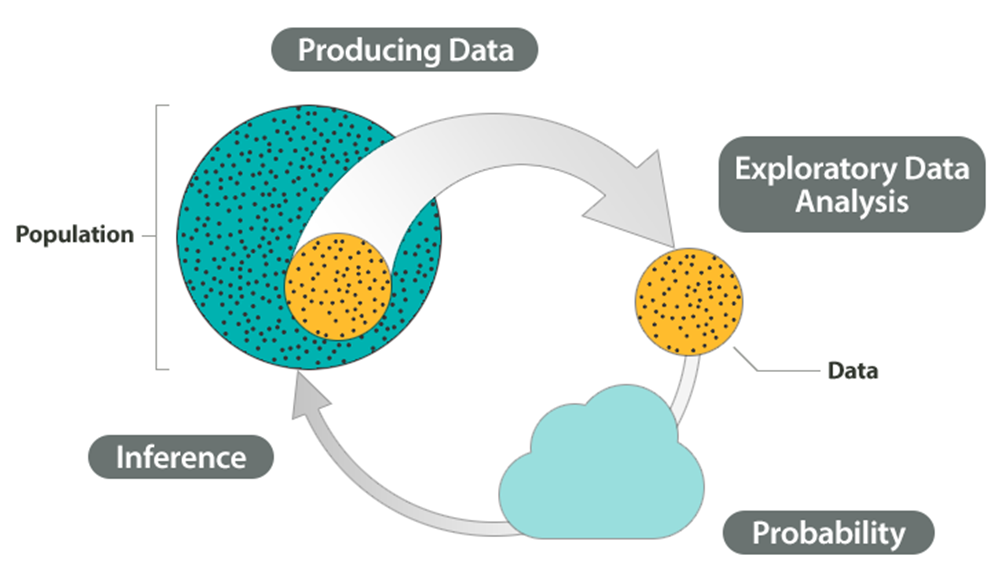
\includegraphics[width=0.68\textwidth]{figures/BigPicture.png}
\end{center}

\vspace{-0.4em}
We have spent the course going \emph{clockwise}: produce data, explore it, model it. \hl{Inference} is the arrow that goes back, from the sample in our hands to the population we care about.

\end{frame}
%%%%%%%%%%%%%%%%%%%%%%%%%%%%%%%%%%%%%%%%%%%%%%%%%%%%%%%%%%%%%%%%%%%%%%%%
\section{Statistics and sampling distributions}
%%%%%%%%%%%%%%%%%%%%%%%%%%%%%%%%%%%%%%%%%%%%%%%%%%%%%%%%%%%%%%%%%%%%%%%%
\begin{frame}
\frametitle{Statistic vs.\ sampling distribution}

\begin{itemize}
\item A \hl{statistic} is a single number computed from one sample:
\[
\widehat{p}, \qquad \bar{x}, \qquad \bar{x}_1 - \bar{x}_2, \qquad \widehat\beta_1 .
\]
\item Its \hl{sampling distribution} is how that statistic varies \emph{across repeated samples} from the same process.
\end{itemize}

\pause
\keyidea[-- The central move]{We only ever see \emph{one} value of the statistic. Inference reasons about the whole distribution it \emph{could} have taken, so the game is to get hold of that distribution.}

\pause
\vspace{-0.5em}
\dq{We cannot repeat the study a thousand times. So how do we get that distribution?}

\end{frame}
%%%%%%%%%%%%%%%%%%%%%%%%%%%%%%%%%%%%%%%%%%%%%%%%%%%%%%%%%%%%%%%%%%%%%%%%
\begin{frame}
\frametitle{The null distribution: one we \emph{can} build}

We cannot sample the real population again. But if we \emph{assume} a specific claim is true, we can simulate from it as often as we like.

\vspace{0.4em}
\begin{center}
\begin{tabular}{lll}
\toprule
Distribution & Repeated under & Used for \\
\midrule
Sampling & the real process & uncertainty in an estimate \\
\hl{Null} & the $H_0$ model & \hl{hypothesis testing} \\
\bottomrule
\end{tabular}
\end{center}

\vspace{0.5em}
\keyidea[-- Null distribution]{The distribution of the test statistic \emph{assuming $H_0$ is true}. A randomization test builds it by simulating a world in which $H_0$ holds, then asks how unusual our real data look.}

\end{frame}
%%%%%%%%%%%%%%%%%%%%%%%%%%%%%%%%%%%%%%%%%%%%%%%%%%%%%%%%%%%%%%%%%%%%%%%%
\section{Hypothesis testing review}
%%%%%%%%%%%%%%%%%%%%%%%%%%%%%%%%%%%%%%%%%%%%%%%%%%%%%%%%%%%%%%%%%%%%%%%%
\begin{frame}
\frametitle{The hypothesis testing procedure}

\begin{enumerate}
\item Choose the parameter of interest.
\item State $H_0$ and $H_A$.
\item Choose a test statistic $T$.
\item Find or \emph{simulate} the null distribution of $T$.
\item Compute the p-value.
\item Interpret the result in context.
\end{enumerate}

\vspace{0.5em}
\caution{Do not start from a p-value. Start from a question and a pair of hypotheses; the p-value is the \emph{last} step, not the first.}

\end{frame}
%%%%%%%%%%%%%%%%%%%%%%%%%%%%%%%%%%%%%%%%%%%%%%%%%%%%%%%%%%%%%%%%%%%%%%%%
\begin{frame}
\frametitle{Null and alternative hypotheses}

\begin{columns}[T]
\column{0.48\textwidth}
\textbf{Null $H_0$}
\begin{itemize}
\item a claim of \emph{no effect} / no difference
\item specific enough to \emph{simulate from}
\end{itemize}

\column{0.48\textwidth}
\textbf{Alternative $H_A$}
\begin{itemize}
\item what we are looking for evidence of
\item one-sided or two-sided
\end{itemize}
\end{columns}

\activity[-- write the hypotheses]{Is the average wait time different from $10$ minutes? Write $H_0$ and $H_A$ using $\mu$.}

\pause
\solnbox{$H_0:\mu=10$ \quad versus \quad $H_A:\mu\neq10$ (two-sided: ``different'' does not say which way).}

\end{frame}
%%%%%%%%%%%%%%%%%%%%%%%%%%%%%%%%%%%%%%%%%%%%%%%%%%%%%%%%%%%%%%%%%%%%%%%%
\begin{frame}
\frametitle{Choosing a test statistic}

The statistic must move in the direction $H_A$ describes.

\vspace{0.3em}
\begin{center}
\begin{tabular}{lll}
\toprule
Question & Parameter & Statistic \\
\midrule
One proportion & $p$ & $\widehat{p}$ \\
One mean & $\mu$ & $\bar{x}$ \\
Two means & $\mu_1-\mu_2$ & $\bar{x}_1-\bar{x}_2$ \\
Two proportions & $p_1-p_2$ & $\widehat{p}_1-\widehat{p}_2$ \\
\bottomrule
\end{tabular}
\end{center}

\vspace{0.5em}
\caution{Choose the statistic \emph{before} you see the simulated p-value. Picking whichever statistic gives the smallest p-value is not a test; it is a search.}

\end{frame}
%%%%%%%%%%%%%%%%%%%%%%%%%%%%%%%%%%%%%%%%%%%%%%%%%%%%%%%%%%%%%%%%%%%%%%%%
\begin{frame}
\frametitle{The p-value}

Let $T_{obs}$ be the value of the statistic we actually observed.

\keyidea[-- p-value]{The probability, \emph{assuming $H_0$ is true}, of getting a statistic at least as extreme as $T_{obs}$.}

\begin{itemize}
\item A small p-value means: \emph{this result would be rare in a world where $H_0$ holds}.
\pause
\item It is \textbf{not} the probability that $H_0$ is true.
\item It is \textbf{not} the size or the importance of the effect.
\item It is \textbf{not} the probability the result was ``due to chance''.
\end{itemize}

\end{frame}
%%%%%%%%%%%%%%%%%%%%%%%%%%%%%%%%%%%%%%%%%%%%%%%%%%%%%%%%%%%%%%%%%%%%%%%%
\begin{frame}
\frametitle{What counts as ``extreme''?}

``At least as extreme'' means \emph{in the direction $H_A$ points}, so $H_A$ decides how we count.

\vspace{-0.1em}
{\footnotesize
\begin{center}
\begin{tabular}{lll}
\toprule
$H_A$ & ``Extreme'' means & Count the simulations with \\
\midrule
$p \neq p_0$ \; (two-sided) & as far from $p_0$, \emph{either way} & $|\widehat{p}_{sim}-p_0| \ge |\widehat{p}_{obs}-p_0|$ \\
$p > p_0$ \; (one-sided) & as far \emph{above} $p_0$ & $\widehat{p}_{sim} \ge \widehat{p}_{obs}$ \\
$p < p_0$ \; (one-sided) & as far \emph{below} $p_0$ & $\widehat{p}_{sim} \le \widehat{p}_{obs}$ \\
\bottomrule
\end{tabular}
\end{center}}

\vspace{-0.2em}
\caution{Choose one-sided or two-sided from the \emph{question}, before seeing the data. The two-sided p-value is about twice the one-sided one; switching afterwards to get the smaller number is cheating.}

\end{frame}
%%%%%%%%%%%%%%%%%%%%%%%%%%%%%%%%%%%%%%%%%%%%%%%%%%%%%%%%%%%%%%%%%%%%%%%%
\begin{frame}
\frametitle{Making a p-value intuitive: the s-value}

A p-value is a small decimal, and small decimals are hard to feel. One fix is the \hl{s-value}:
\[
\text{s-value} := -\log_2(\text{p-value}).
\]
\pause
\hl{Read it as:} how many \emph{heads in a row} would be about this surprising?
\[
P(k\text{ heads in a row}) = \left(\tfrac12\right)^{k} \approx p
\quad\Longrightarrow\quad
k \approx -\log_2(p).
\]
\pause
\vspace{-0.5em}
{\footnotesize
\begin{center}
\begin{tabular}{rcccc}
\toprule
p-value & $0.10$ & $0.05$ & $0.01$ & $0.001$ \\
\midrule
s-value (heads in a row) & $3.3$ & $4.3$ & $6.6$ & $10.0$ \\
\bottomrule
\end{tabular}
\end{center}}

\ct{Greenland, S. (2019). Valid P-Values Behave Exactly as They Should. \emph{Am.\ Stat.} \textbf{73}, 106--114.}

\end{frame}
%%%%%%%%%%%%%%%%%%%%%%%%%%%%%%%%%%%%%%%%%%%%%%%%%%%%%%%%%%%%%%%%%%%%%%%%
\begin{frame}
\frametitle{From p-value to decision}

Fix a significance level $\alpha$ \emph{in advance}, then
\[
\text{reject } H_0 \quad\text{if}\quad p\text{-value} < \alpha .
\]
\vspace{0.3em}
{\small
\begin{center}
\begin{tabular}{lll}
\toprule
Decision & Means & Does \emph{not} mean \\
\midrule
Reject $H_0$ & evidence against $H_0$ & $H_A$ is certain \\
Do not reject $H_0$ & insufficient evidence & $H_0$ is true \\
\bottomrule
\end{tabular}
\end{center}}

\vspace{0.4em}
\caution{Failing to reject is not proof of no effect; it may just mean the sample was too small to see one. \emph{Absence of evidence is not evidence of absence.}}

\end{frame}
%%%%%%%%%%%%%%%%%%%%%%%%%%%%%%%%%%%%%%%%%%%%%%%%%%%%%%%%%%%%%%%%%%%%%%%%
\begin{frame}
\frametitle{Decision errors}

We decide from one sample, so we can be wrong two ways:

\begin{center}
\begin{tabular}{l|cc}
& \multicolumn{2}{c}{\textbf{Truth}} \\
\textbf{Decision} & $H_0$ true & $H_A$ true \\
\hline
Reject $H_0$ & \hl{Type I error} & correct \\
Do not reject $H_0$ & correct & \hl{Type II error} \\
\end{tabular}
\end{center}

\vspace{0.5em}
\begin{itemize}
\item \textbf{Type I} (false positive): we ``find'' an effect that is not there. Its rate is exactly what $\alpha$ controls.
\item \textbf{Type II} (false negative): a real effect we failed to detect.
\item \hl{Power} $=1-P(\text{Type II error})$: the chance of \emph{catching} a real effect. It rises with the sample size and with the size of the effect.
\end{itemize}

\end{frame}
%%%%%%%%%%%%%%%%%%%%%%%%%%%%%%%%%%%%%%%%%%%%%%%%%%%%%%%%%%%%%%%%%%%%%%%%
\begin{frame}
\frametitle{Activity: errors in context}

\activity[-- spam filter]{%
A spam filter flags an email as spam when the test rejects $H_0$: ``this email is \emph{not} spam''.

\begin{enumerate}
\item What is a Type I error, in plain language?
\item What is a Type II error?
\item Which is worse for a personal inbox? For a corporate security system?
\end{enumerate}}
\end{frame}
%%%%%%%%%%%%%%%%%%%%%%%%%%%%%%%%%%%%%%%%%%%%%%%%%%%%%%%%%%%%%%%%%%%%%%%%
\begin{frame}
\frametitle{Activity: errors in context}
\solnbox{(1) A real email is sent to the junk folder. (2) A spam email lands in your inbox. (3) Personal inbox: Type I is worse (losing a real email beats deleting one spam). Corporate security: Type II is worse (one phishing email getting through can be catastrophic). \emph{Same test, opposite priorities.}}

\end{frame}
%%%%%%%%%%%%%%%%%%%%%%%%%%%%%%%%%%%%%%%%%%%%%%%%%%%%%%%%%%%%%%%%%%%%%%%%
\section{Randomization tests}
%%%%%%%%%%%%%%%%%%%%%%%%%%%%%%%%%%%%%%%%%%%%%%%%%%%%%%%%%%%%%%%%%%%%%%%%
\begin{frame}
\frametitle{Randomization test: the core idea}

\keyidea[-- The whole trick]{If we can \emph{simulate} a world where $H_0$ is true, we can build the null distribution by brute force, with no formula required.}

\begin{enumerate}
\item Compute the observed statistic $T_{obs}$ from the real data.
\item Generate $B$ datasets \emph{as if $H_0$ were true} (we will use $B=10{,}000$).
\item Recompute the statistic on each one.
\item The p-value is the fraction of those $B$ statistics at least as extreme as $T_{obs}$.
\end{enumerate}

\vspace{0.3em}
The p-value is literally a \emph{proportion we count}.

\end{frame}
%%%%%%%%%%%%%%%%%%%%%%%%%%%%%%%%%%%%%%%%%%%%%%%%%%%%%%%%%%%%%%%%%%%%%%%%
\begin{frame}
\frametitle{What do we randomize?}

Whatever $H_0$ says is \hl{exchangeable} --- i.e.\ what could have come out differently if $H_0$ were true.

\begin{center}
{\small
\begin{tabular}{ll}
\toprule
Null claim & What to randomize \\
\midrule
$p = p_0$ & generate Bernoulli($p_0$) outcomes \\
No group effect & \hl{permute the group labels} \\
No paired difference & swap labels within each pair \\
No regression relationship & permute the response values \\
\bottomrule
\end{tabular}}
\end{center}

\vspace{-0.1em}
\caution{Randomize the wrong thing and you test the wrong null hypothesis. Ask first: \emph{if $H_0$ were true, what could have been shuffled without changing anything?}}

\end{frame}
%%%%%%%%%%%%%%%%%%%%%%%%%%%%%%%%%%%%%%%%%%%%%%%%%%%%%%%%%%%%%%%%%%%%%%%%
\begin{frame}
\frametitle{Step-by-step: a complete randomization test}

\examplehead{Office hours}

We survey $n=40$ students; $29$ say they prefer \emph{online} office hours.

\begin{enumerate}
\item \textbf{Parameter:} $p$, the true proportion who prefer online.
\pause
\item \textbf{Hypotheses:} $H_0:p=0.5$ \; vs \; $H_A:p\neq0.5$.
\pause
\item \textbf{Statistic:} $\widehat{p}$. \quad Observed: $\widehat{p}_{obs}=29/40=\hl{0.725}$.
\pause
\item \textbf{Simulate the null:} if $H_0$ held, each student is a coin flip, so draw $40$ Bernoulli($0.5$) outcomes and recompute $\widehat{p}$. Repeat $10{,}000$ times.
\pause
\item \textbf{Count:} what fraction of those $10{,}000$ landed at least as far from $0.5$ as $0.725$ did?
\end{enumerate}

\end{frame}
%%%%%%%%%%%%%%%%%%%%%%%%%%%%%%%%%%%%%%%%%%%%%%%%%%%%%%%%%%%%%%%%%%%%%%%%
\begin{frame}
\frametitle{The null distribution \emph{is} the p-value}

\begin{center}
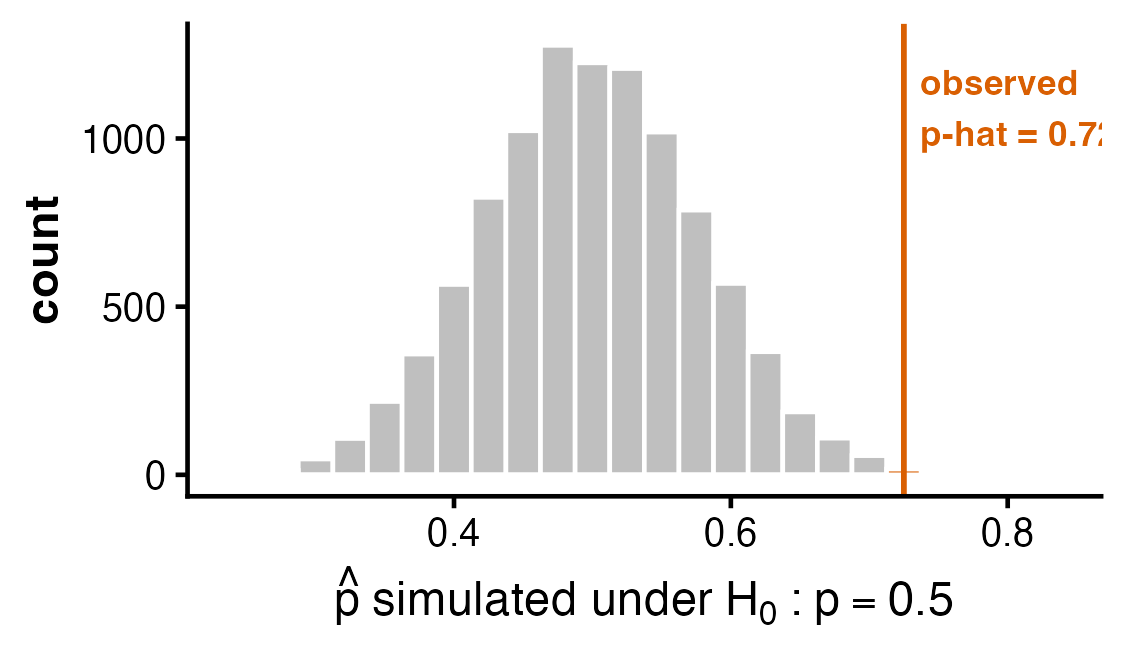
\includegraphics[width=0.76\textwidth]{figures/null-dist-proportion.png}
\end{center}

\vspace{-0.7em}
\pause
\textbf{Step 6 --- interpret:} if students really split $50/50$, a sample this lopsided would arise only about $0.5\%$ of the time, about as surprising as $7$ or $8$ heads in a row. Strong evidence against $H_0$.

\end{frame}
%%%%%%%%%%%%%%%%%%%%%%%%%%%%%%%%%%%%%%%%%%%%%%%%%%%%%%%%%%%%%%%%%%%%%%%%
\begin{frame}[fragile]
\frametitle{Doing it in R}

\begin{lstlisting}[language=R]
n <- 40; p0 <- 0.5
phat_obs <- 29 / 40          # 0.725

# simulate a world where H0 is true
phat_null <- replicate(10000,
  mean(rbinom(n, 1, p0)))

mean(abs(phat_null - p0) >=
     abs(phat_obs - p0))     #> 0.005
\end{lstlisting}

\vspace{0.3em}
The last line \emph{is} the definition of the p-value: the proportion of simulated statistics at least as far from $p_0$ as ours.

\end{frame}
%%%%%%%%%%%%%%%%%%%%%%%%%%%%%%%%%%%%%%%%%%%%%%%%%%%%%%%%%%%%%%%%%%%%%%%%
\begin{frame}
\frametitle{Example 2: two groups (permute the labels)}

\examplehead{Two teaching methods}

Two sections take the same quiz ($n=30$ each):
\[
\bar{x}_A = 79.67,
\qquad
\bar{x}_B = 75.06,
\qquad
T_{obs}=\bar{x}_A-\bar{x}_B=\hl{4.61}.
\]
\vspace{0.2em}
$H_0:\mu_A=\mu_B$ \; vs \; $H_A:\mu_A\neq\mu_B$.

\keyidea[-- Exchangeability]{If the method truly had no effect, a student's score would have been the same whichever section they landed in. So the \emph{labels} carry no information, and we can shuffle them, keeping the scores and group sizes fixed.}

\end{frame}
%%%%%%%%%%%%%%%%%%%%%%%%%%%%%%%%%%%%%%%%%%%%%%%%%%%%%%%%%%%%%%%%%%%%%%%%
\begin{frame}
\frametitle{The permutation null distribution}

Shuffle the labels $10{,}000$ times, recomputing $\bar{x}_A-\bar{x}_B$ each time:

\begin{center}
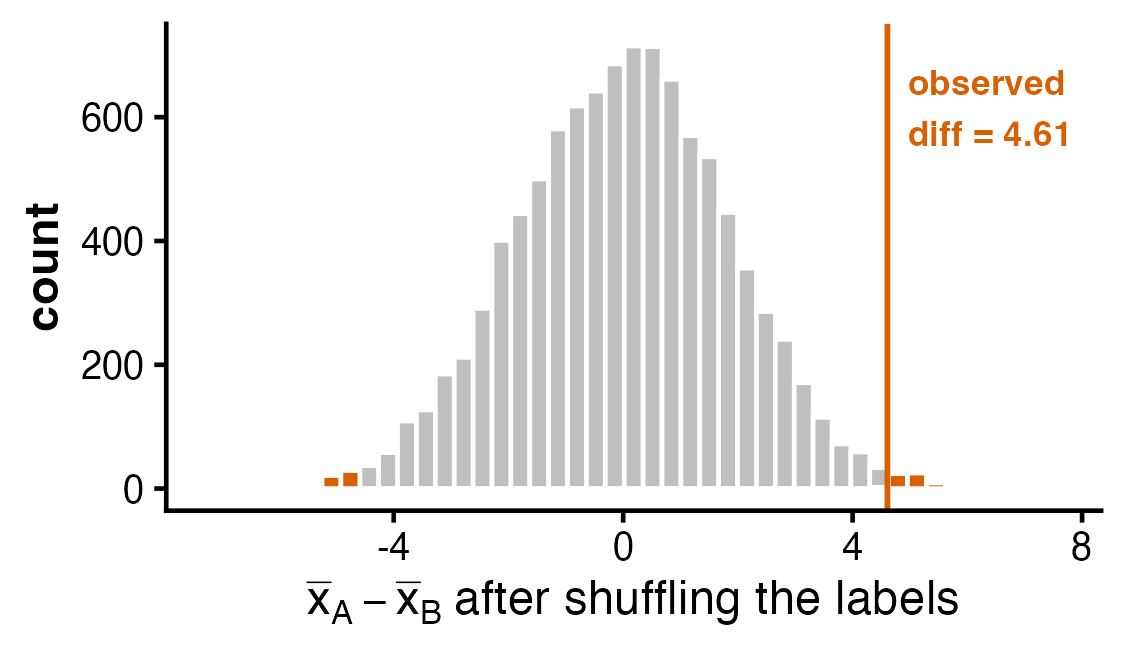
\includegraphics[width=0.74\textwidth]{figures/null-dist-permutation.png}
\end{center}

\vspace{-0.7em}
\pause
Only $1.4\%$ of shuffles produce a gap this large, so $p=0.014$: \textbf{evidence the two methods really do differ}.

\end{frame}
%%%%%%%%%%%%%%%%%%%%%%%%%%%%%%%%%%%%%%%%%%%%%%%%%%%%%%%%%%%%%%%%%%%%%%%%
\begin{frame}[fragile]
\frametitle{Permuting labels in R}

\begin{lstlisting}[language=R]
obs <- mean(score[group=="A"]) -
       mean(score[group=="B"])   # 4.61
diff_null <- replicate(10000, {
  shuffled <- sample(group)  # shuffle!
  mean(score[shuffled=="A"]) -
    mean(score[shuffled=="B"])
})
mean(abs(diff_null) >= abs(obs))  #> .014
\end{lstlisting}

\vspace{-0.4em}
\caution{Shuffle the \emph{labels}, not the scores, and keep the group sizes fixed.}

\end{frame}
%%%%%%%%%%%%%%%%%%%%%%%%%%%%%%%%%%%%%%%%%%%%%%%%%%%%%%%%%%%%%%%%%%%%%%%%
\begin{frame}
\frametitle{How many simulations is enough?}

\vspace{-0.3em}
\begin{center}
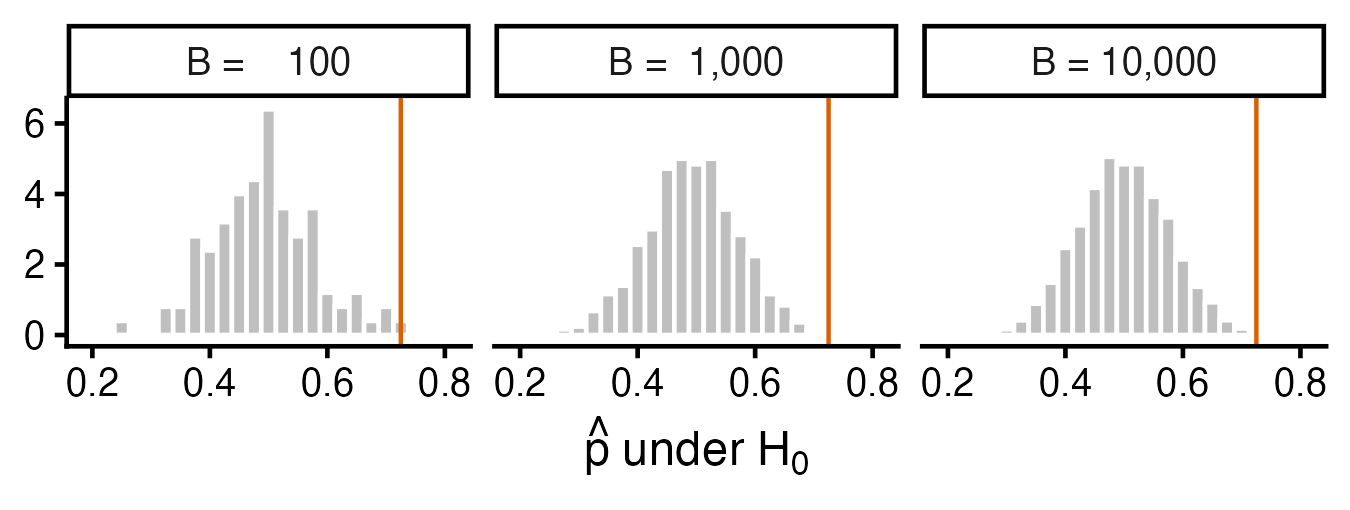
\includegraphics[width=0.68\textwidth]{figures/how-many-sims.png}
\end{center}

\vspace{-1.1em}
The \emph{shape} settles fast; the \emph{p-value} wobbles while $B$ is small:

\vspace{-0.4em}
{\footnotesize
\begin{center}
\begin{tabular}{lccccc}
\toprule
$B$ & 100 & 1{,}000 & 10{,}000 & 50{,}000 & \textbf{exact} \\
\midrule
p-value & \hl{0.000} & 0.006 & 0.006 & 0.007 & \textbf{0.0064} \\
\bottomrule
\end{tabular}
\end{center}}
\vspace{-0.5em}

\vspace{-0.4em}
\caution{At $B=100$ we got $p=\mathbf{0}$, but a simulated p-value is \emph{never} truly zero. It only means ``smaller than $1/B$''. Report $p<1/B$.}

\end{frame}
%%%%%%%%%%%%%%%%%%%%%%%%%%%%%%%%%%%%%%%%%%%%%%%%%%%%%%%%%%%%%%%%%%%%%%%%
\begin{frame}
\frametitle{Common mistakes}

\begin{itemize}
\item Simulating from the \emph{observed} proportion instead of the null value $p_0$.
\item Shuffling the outcomes when $H_0$ says the \emph{labels} are exchangeable.
\item Letting the group sizes change when permuting.
\item Reading the p-value as $P(H_0\text{ true})$.
\item Treating statistical significance as practical importance.
\end{itemize}

\vspace{0.5em}
\caution{Before you simulate, answer one question: \emph{if $H_0$ were true, what exactly could have come out differently?} That answer is what you randomize.}

\end{frame}
%%%%%%%%%%%%%%%%%%%%%%%%%%%%%%%%%%%%%%%%%%%%%%%%%%%%%%%%%%%%%%%%%%%%%%%%
\section{Activity}
%%%%%%%%%%%%%%%%%%%%%%%%%%%%%%%%%%%%%%%%%%%%%%%%%%%%%%%%%%%%%%%%%%%%%%%%
\begin{frame}
\frametitle{Activity: design the test before you run it}

\activity[-- in pairs]{%
For each scenario give: (1) the parameter, (2) $H_0$ and $H_A$, (3) the statistic, (4) \emph{what you would randomize}, (5) how you would get the p-value.

\smallskip
\textbf{A.} Of $80$ students surveyed, $50$ prefer online office hours. Is the true rate above $50\%$?

\smallskip
\textbf{B.} Two independent discussion sections sit the same quiz. Do their mean scores differ?}

\end{frame}
%%%%%%%%%%%%%%%%%%%%%%%%%%%%%%%%%%%%%%%%%%%%%%%%%%%%%%%%%%%%%%%%%%%%%%%%
\begin{frame}
\frametitle{Activity: design the test before you run it}
{\small
\solnbox{\textbf{A:} $p$; $H_0:p=0.5$ vs $H_A:p>0.5$; $\widehat p=50/80=0.625$; \emph{simulate} $80$ Bernoulli($0.5$) draws; p-value $=$ fraction with $\widehat p \ge 0.625$.
\textbf{B:} $\mu_A-\mu_B$; $H_0:\mu_A=\mu_B$ vs $H_A:\mu_A\neq\mu_B$; $\bar x_A-\bar x_B$; \emph{permute} the labels; p-value $=$ fraction with $|$shuffled diff$| \ge |$observed$|$.}}

\end{frame}
%%%%%%%%%%%%%%%%%%%%%%%%%%%%%%%%%%%%%%%%%%%%%%%%%%%%%%%%%%%%%%%%%%%%%%%%
\begin{frame}
\frametitle{Why were the two methods different?}

\begin{center}
\begin{tabular}{lcc}
\toprule
Scenario & Simulate from $H_0$? & Permute labels? \\
\midrule
One proportion & \hl{yes} & no \\
Two groups & no & \hl{yes} \\
\bottomrule
\end{tabular}
\end{center}

\vspace{0.5em}
\dq{Why does the randomization method differ between the two?}

\end{frame}
%%%%%%%%%%%%%%%%%%%%%%%%%%%%%%%%%%%%%%%%%%%%%%%%%%%%%%%%%%%%%%%%%%%%%%%%
\begin{frame}
\frametitle{Why were the two methods different?}
\solnbox{Because the nulls say different things. ``$p=0.5$'' names a \emph{mechanism} we can generate from directly. ``No group effect'' names no mechanism at all: it only says the labels are meaningless, so we impose it by \emph{scrambling the labels} and keeping the data.}

\end{frame}
%%%%%%%%%%%%%%%%%%%%%%%%%%%%%%%%%%%%%%%%%%%%%%%%%%%%%%%%%%%%%%%%%%%%%%%%
\section{Wrap-up}
%%%%%%%%%%%%%%%%%%%%%%%%%%%%%%%%%%%%%%%%%%%%%%%%%%%%%%%%%%%%%%%%%%%%%%%%
\begin{frame}
\frametitle{Key takeaways}

\begin{itemize}
\item Start from a question; state $H_0$ and $H_A$ first.
\item Pick a statistic that moves the way $H_A$ says.
\item Ask: \emph{if $H_0$ were true, what could have come out differently?} Randomize that.
\item Simulate many times to build the \hl{null distribution}.
\item The \hl{p-value} is the fraction of simulations at least as extreme as what you saw.
\item Interpret in context, and remember which \emph{error} you would rather make.
\end{itemize}

\vspace{-0.1em}
\caution{A randomization test is not a button in R. It is a model of what ``no effect'' would look like.}

\end{frame}
%%%%%%%%%%%%%%%%%%%%%%%%%%%%%%%%%%%%%%%%%%%%%%%%%%%%%%%%%%%%%%%%%%%%%%%%

%%%%%%%%%%%%%%%%%%%%%%%%%%%%%%%%%%%%
% End document
%%%%%%%%%%%%%%%%%%%%%%%%%%%%%%%%%%%%

\end{document}
